\documentclass{ExamCUNY}
\usepackage{mathrsfs}
\usepackage{stix}
\usepackage{pgffor}
\usepackage{bm}
\usepackage{microtype}
\usepackage{nicematrix}
\usepackage{booktabs}
\usepackage{mathtools}
\usepackage{tikz}
\usetikzlibrary{calc, 3d, automata, positioning, arrows.meta}

\usepackage{tabstackengine}
\TABstackMath
\TABbinary

\ExamNumber{1}%
\CourseName{Automation Engineering}
\CourseNumber{39531}
\InstructorName{Alex Washburn}
\DueDateYear{2026}
\DueDateMonth{03}
\DueDateDay{06}

\newcommand{\?}{\stackrel{?}{=}}
\newcommand{\R}[2]{\ensuremath{\World{#1}\mathrel{R}\World{#2}}\xspace}
\newcommand{\Tr}[2]{\ensuremath{\tau\Parens{#1,\,#2}\xspace}}
\newcommand{\T}[1]{\ensuremath{\tau\Parens{#1}\xspace}}
\newcommand{\Prob}[1]{\ensuremath{P\Parens{#1}}\xspace}
\newcommand{\ProbGiven}[2]{\ensuremath{P\Parens{#1\,|\,#2}}\xspace}
\newcommand{\Event}[1]{\ensuremath{\bm{\mathsf{#1}}}\xspace}
\newcommand{\RandVar}[1]{\ensuremath{\mathbf{#1}}\xspace}
\newcommand{\DistMap}[2]{~#1&\mapsto~~#2\\}
\newcommand{\DistCondition}[2]{~#1&\text{\normalfont iff}~~#2\\}

\newcommand{\Hint}[1]{\textit{\textls{Hint:}~#1}}

\newcommand{\One}{\ensuremath{\textbf{1}}\xspace}

\newcommand{\EquivGrid}{\ensuremath{~\;\;\equiv\quad}\xspace}

\newcommand{\Coin}[1]{\ensuremath{\mathbf{C}_{#1}}\xspace}
\newcommand{\CoinBiased}[1]{\ensuremath{\mathscr{C}_{#1}}\xspace}
\newcommand{\Heads}{\ensuremath{\mathtt{H}}\xspace}
\newcommand{\Tails}{\ensuremath{\mathtt{T}}\xspace}

\newcommand{\Die}[1]{\ensuremath{\mathbf{D}_{#1}}\xspace}
\newcommand{\Above}[1]{\ensuremath{\overline{#1}}\xspace}
\newcommand{\Below}[1]{\ensuremath{\underline{#1}}\xspace}
\newcommand{\Num}[1]{\ensuremath{\mathbb{#1}}\xspace}
\newcommand{\NumA}[1]{\ensuremath{\overline{\Num{#1}}}\xspace}
\newcommand{\NumB}[1]{\ensuremath{\underline{\Num{#1}}}\xspace}

\newcommand{\Deck}{\ensuremath{\bm{\mathcal{D}}}\xspace}
\newcommand{\CardSuits}{\ensuremath{\bm{\mathcal{S}}}\xspace}
\newcommand{\CardRanks}{\ensuremath{\bm{\mathcal{R}}}\xspace}
\newcommand{\CardRank}[1]{\ensuremath{\text{\textsf{\textbf{#1}}}}\xspace}


\newcommand{\Countermodel}[4]{%
\textbf{Countermodel} $\mathcal{K}$ in #1:%
\begin{itemize}%
\item \ensuremath{W = \SetNote{\World{0}%
\foreach \n in {1,...,#2}{,~\World{\n}}%
}}%
\item \ensuremath{\mathrel{R}~=~#3}%
\item #4%
\end{itemize}%
}

\begin{document}
\CoverPage%

\newcommand{\BulletLong}[3]{\hspace*{4mm}\ensuremath{\Parens{\Event{#1}}}:\hspace*{2mm}#2\[#3\]\\[5mm]}
\newcommand{\BulletLine}[3]{\hspace*{4mm}\ensuremath{\Parens{\Event{#1}}}:\hspace*{2mm}#2\hfill\ensuremath{#3}\\[5mm]}
\newcommand{\Bullet}[2]{\hspace*{4mm}\ensuremath{\Parens{\Event{#1}}}:\hspace*{2mm}#2\\[5mm]}

\newcommand{\True}{\ensuremath{\bm{\mathtt{True}}}\xspace}
\newcommand{\False}{\ensuremath{\bm{\mathtt{False}}}\xspace}

\newcommand{\TrueFalse}[1]{\ensuremath{\True\;\oplus\;\False\;\colon~~{#1}}}
\newcommand{\TrueFALSE}[1]{\ensuremath{\True\;\oplus\;\underline{\False}\;\colon~~{#1}}}
\newcommand{\TRUEFalse}[1]{\ensuremath{\underline{\True}\;\oplus\;\False\;\colon~~{#1}}}

\newcommand{\SupportFalsify}[1]{\ensuremath{\mathtt{Support}\;\leftrightarrow\;\mathtt{Falsify}\;\colon}~~{#1}}
\newcommand{\SupportFALSIFY}[1]{\ensuremath{\mathtt{Support}\;\leftrightarrow\;\underline{\mathtt{Falsify}}\;\colon~~{#1}}}


\newcommand{\Bc}{\cellcolor{blue!20}}



\newcommand{\Reals}{\ensuremath{\mathbb{R}}\xspace}
\newcommand{\PMF}[2]{%
\expandafter\ifx\expandafter\relax%
\detokenize{#2}\relax\ensuremath{\rho_{{\textstyle\mathstrut}\RandVar{#1}}}\xspace\else\ensuremath{\rho_{{\textstyle\mathstrut}\RandVar{#1}}\Parens{#2}}\xspace\fi}

\newcommand{\PDF}[2]{%
\expandafter\ifx\expandafter\relax%
\detokenize{#2}\relax\ensuremath{\mathit{f}_{{\textstyle\mathstrut}\RandVar{#1}}}\xspace\else\ensuremath{\mathit{f}_{\RandVar{{\textstyle\mathstrut}#1}}\Parens{#2}}\xspace\fi}

\newcommand{\Expect}[1]{\ensuremath{\mathbb{E}\left[\,#1\,\right]}\xspace}
\newcommand{\Variance}[1]{\ensuremath{\mathtt{Var}\Parens{#1}}\xspace}

%%%%%%%%%%%%%
% Instructions
\newcommand{\Q}[1]{\ensuremath{\textbf{Question #1}}\xspace}

\clearpage%
\newgeometry{bottom=20mm,left=20mm,right=20mm,top=20mm}%
\begin{center}
{\Huge \underline{Examination Instructions}}
\end{center}
~\vspace*{5mm}
{\Large
\begin{itemize}
\item Read each question carefully, preferably twice.
\item If you do not understand a question, email to ask for clarification.
\item There are no ``trick questions.''\\
The most straight-forward interpretation of the problem statement is likely the correct interpretation.
\item Show as much of your work and thought process as possible.\\
Partial credit will be given for partially correct answers.
\item I am looking to \emph{give} credit for correctness, not \emph{deduct} credit for mistakes.\\
It is \emph{always better} to be more verbose than to be terse, since you will receive full credit as long some of your solution correctly conveys the answer.
\vspace*{5cm}
\begin{center}
{\Huge \underline{Examination Scoring}}
\end{center}
\begin{align*}
\textit{\textbf{Final Score}}\; &= \Q{1}\\
&\,+ \Q{2}\\
&\,+ \Q{3}\\
&\,+ \Q{4}\\
&\,+ \Q{5}
\end{align*}
\end{itemize}
}



\newcommand{\ExamObject}[2]{%
{\Large \underline{\textbf{|~#1}}}\\[5mm]%
{\Large #2}\\[5mm]%
}

\clearpage%

\Problem{20}{Definitions}{%
Describe, to the best of your ability, the definition of each process automation concept.
You may use the English language, mathematical notation, or some combination of both.
}

\SubProblem{4}{What is a Functor?}
\vfill


\SubProblem{4}{What is a \texttt{fold} function?}
\vfill


\SubProblem{4}{What is a constraint class, and why is it useful?}
\vfill


\SubProblem{4}{What is a Finite State Automata?}
\vfill


\SubProblem{4}{What is a process (to be automated)?}
\vfill


\Problem{20}{Support or Falsify}{%
Consider each statement and regarding the following functions,\\and \textit{either}:\\[5mm]
$$\mathtt{silly} \colon \mathbb{N} \to \mathbb{N} \to \mathbb{N} \to \mathbb{Q}\phantom{\texttt{11111}}$$
$$\mathtt{silly}\Parens{a,\,b,\,c}\;= \frac{a * a}{b + c} - b * c$$
\large
\Bullet{Support}{State that it is $\mathtt{True}$. Explain the reason why you believe that is the case. If you feel capable of providing a proof or a sketch/outline of a proof, please do so.}
\Bullet{Falsify}{State that it is $\mathtt{False}$. Explain the reason why you believe that is the case. If you have a counterexample which shows that the statement is false, please provide it.}
}

\SubProblem{5}{\SupportFalsify{$\mathtt{silly}\Parens{5}$ has type $\mathbb{N} \to \mathbb{Q}$}}
\vfill


\SubProblem{5}{\SupportFalsify{$\mathtt{silly}\Parens{6,\,6} = \Parens{\frac{6}{\Parens{6 - c}}} - c$}}
\vfill


\SubProblem{5}{\SupportFalsify{The value of $\mathtt{silly}\Parens{7,\,0,\,0}$ is in the domain $\mathbb{Q}$}}
\vfill

\SubProblem{5}{\SupportFalsify{$\lambda\Parens{x,y} \to \mathtt{silly}\Parens{y,\,x,\,y} * \mathtt{silly}\Parens{x,\,y,\,x}$ has type $\mathbb{N} \to \mathbb{N} \to \mathbb{Q}$}}
\vfill


\Problem{20}{Problem 1}{%
Consider each statement and regarding the following data-type:\\[5mm]
\begin{equation*}
\linespread{3em}
\mathtt{These}\; \alpha \; \beta \;= \begin{cases}%
\mathtt{None}\\
\mathtt{Left}\; \alpha\\
\mathtt{Right}\; \beta\\
\mathtt{Both}\; \alpha \; \beta
\end{cases}
\end{equation*}
}

\SubProblem{10}{Write an definition of $\oplus \colon \mathtt{These}\; \alpha\; \beta \to \mathtt{These}\; \alpha\; \beta \to \mathtt{These}\; \alpha\; \beta$ which satisfies the \texttt{Semigroup} contraint class \textit{(No proof necessary)}.}
\vfill

\SubProblem{10}{Is there an identety element for your definition of $\oplus$ satisfying the \texttt{Monoid} contraint class? If so, state the identedty element \textit{(No proof necessary)}.}
\vfill


\Problem{20}{Problem 2}{%
MacroSlop  wants to automate its employee expense reimbursement process.
Currently, employees email receipts to their manager.
The manager reviews them and forwards approved expenses to accounting.
Accounting enters the expenses into the finance system and issues reimbursement in the next payroll cycle.
The company wants a new automated system where employees upload receipts, managers approve them if necessary, and reimbursements happen automatically.
Expense approval is only required by a manager only if it exceeds \$100.\\[5mm]
\textit{Use the following data-types to help MacroSlop automate thier employee expense reimbursement process.}
\begin{equation*}
\mathtt{IntakeStatus}\;= \begin{cases}%
\mathtt{ApprovalAutomatic}\; \mathtt{ExpenseID}\\
\mathtt{ApprovalRequired}\phantom{\mathtt{c}}\; \mathtt{ExpenseID}
\end{cases}
\end{equation*}
\begin{equation*}
\mathtt{Approval} \;= \begin{cases}%
\mathtt{ApprovalReceived}\; \mathtt{ExpenseID}\\
\mathtt{ApprovalReject}\phantom{\mathtt{ed}}\; \mathtt{ExpenseID}
\end{cases}
\end{equation*}
}


\SubProblem{10}{Write the function $\mathtt{intakeExpense} \colon \mathtt{ExpenseID} \to \mathtt{US\_Dollars} \to \mathtt{Intake}$, which is the first step of the automation process.}
\vfill

\SubProblem{10}{You can disperse a reimbursment by calling $\mathtt{sendFunds} \colon \mathtt{ExpenseID} \to \mathtt{Void}$. You can always create the value $\mathtt{finish} \colon \mathtt{Void}$. Using these functions, write the function $processExpense \colon \mathtt{Approval} \to \mathtt{Void}$ which is the last step of the automation process.}
\vfill

\Problem{20}{Problem 3}{%
The NYSE has ``circuit breaker'' mechanisms integrated into the trading floor to halt trading if the S\&P 500 index decreases in value under scertain scenarios.
On the following page is a Finite State Automata diagram of the NYSE circuit breakers.
Study the diagram to answer the following questions.
}

\SubProblem{5}{What occurs when S\&P 500 index decreases by 7\%?}
\vfill

\SubProblem{5}{What occurs when S\&P 500 index decreases by 7\% and then additionally decreases by another 6\%?}
\vfill

\SubProblem{5}{What occurs when S\&P 500 index decreases by 7\%, increases by 10\%, then decreases by 6\%?}
\vfill

\SubProblem{5}{When does trading stop for the rest of the day?}
\vfill


\pagebreak
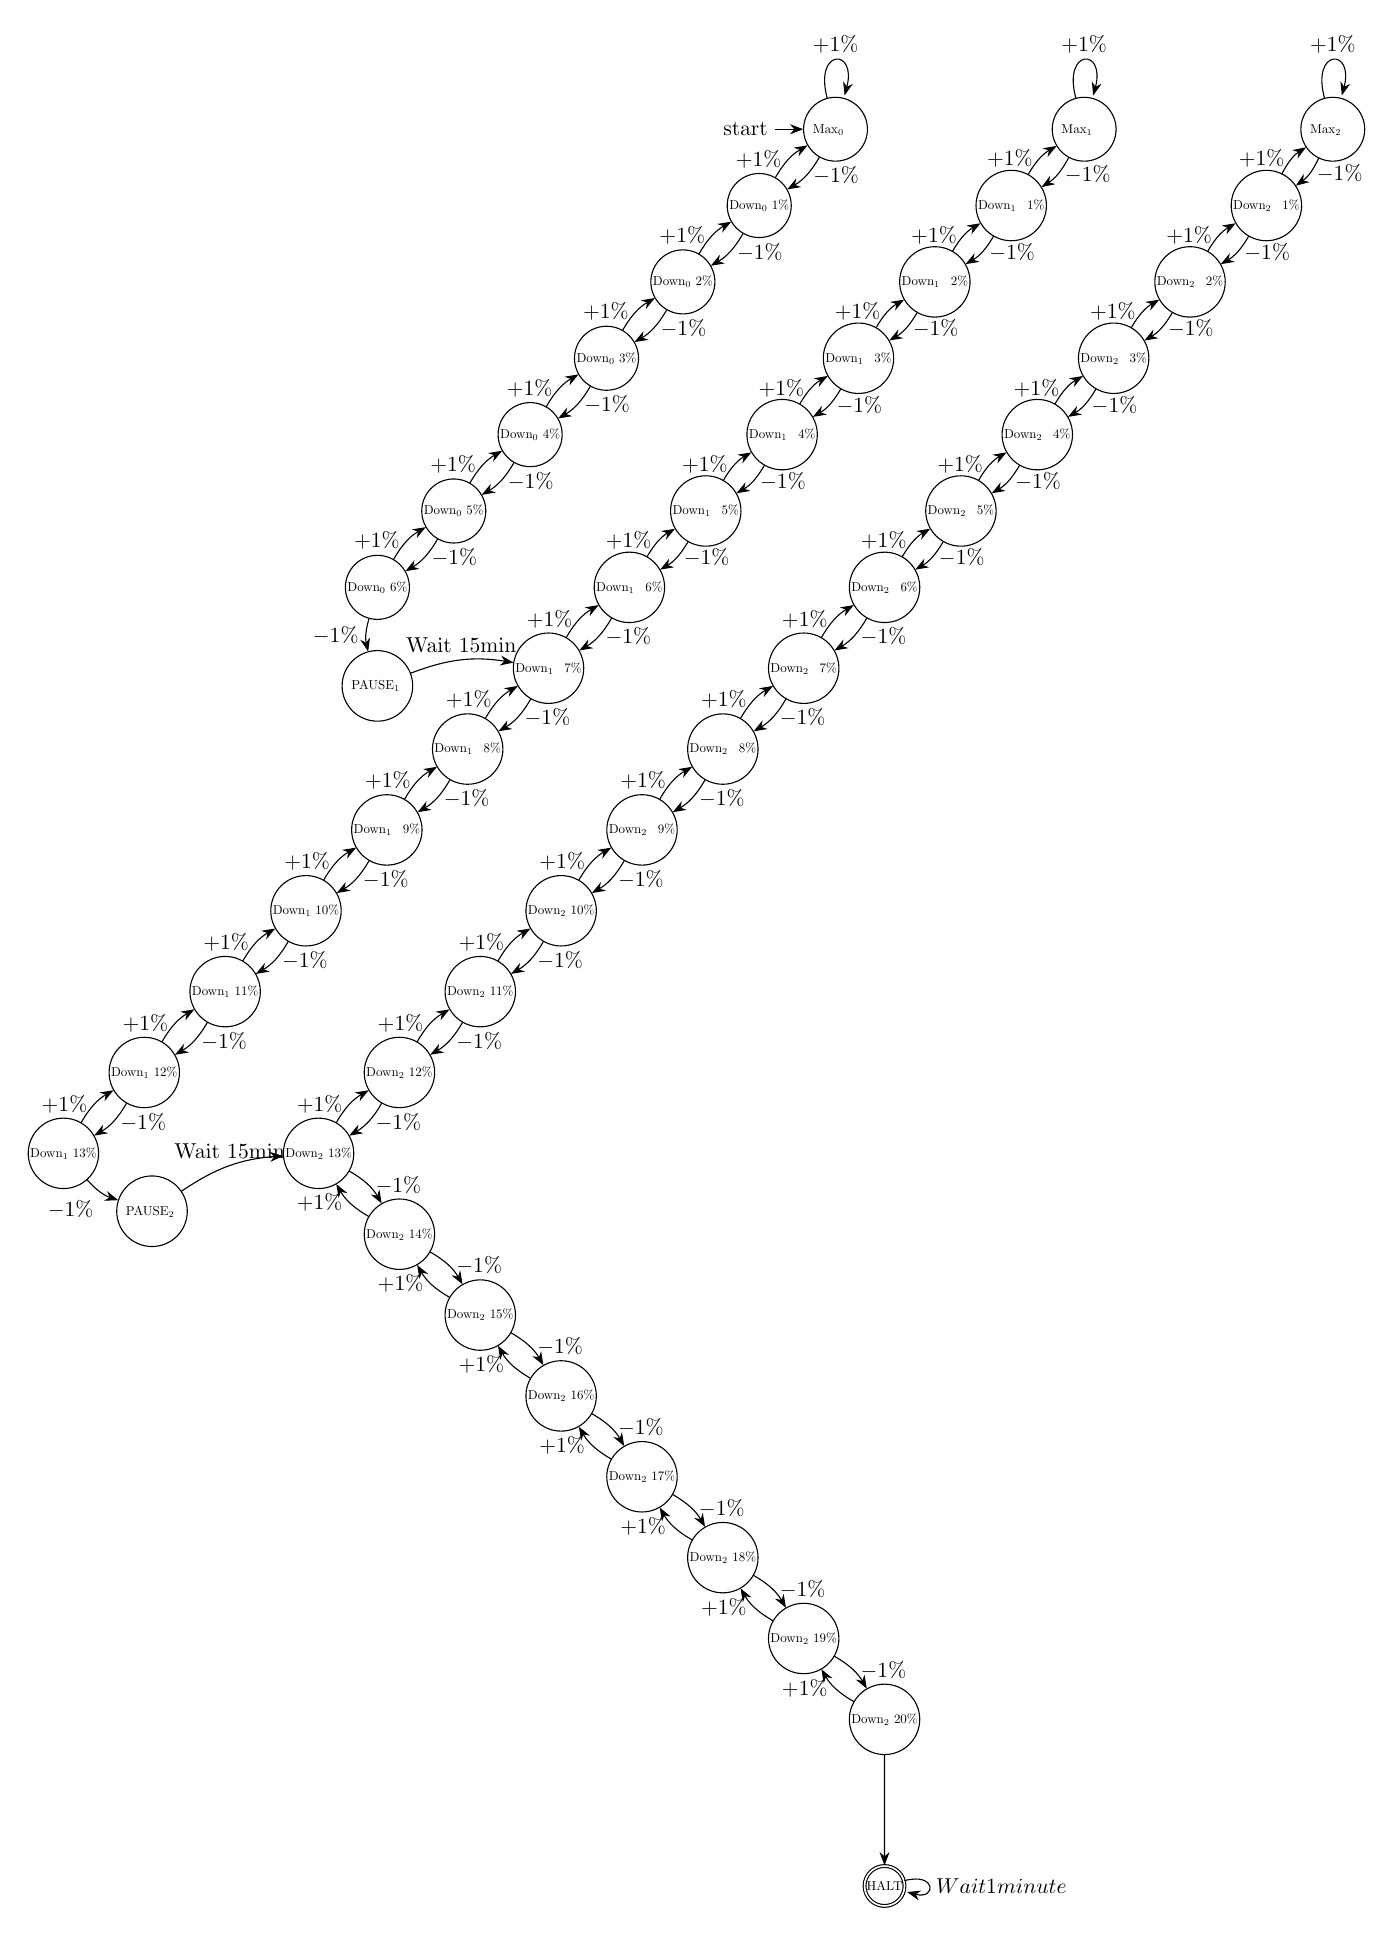
\begin{tikzpicture}[
  >=Stealth,
  node distance=0.75cm,
  auto,
  scale=0.78,
  transform shape
]
\tikzstyle{every state}=[draw=black, minimum size=0.55cm, inner sep=1pt,scale=0.6, every node/.style={scale=0.6}]

% ================= COLUMN A =================
\node[state, initial] (A0) {\phantom{n}$\text{Max}_0$ \phantom{1\%}};
\node[state] (A1) [below left =0.5cm and 0.5cm of A0] {$\text{Down}_{0}$ 1\%};
\node[state] (A2) [below left =0.5cm and 0.5cm of A1] {$\text{Down}_{0}$ 2\%};
\node[state] (A3) [below left =0.5cm and 0.5cm of A2] {$\text{Down}_{0}$ 3\%};
\node[state] (A4) [below left =0.5cm and 0.5cm of A3] {$\text{Down}_{0}$ 4\%};
\node[state] (A5) [below left =0.5cm and 0.5cm of A4] {$\text{Down}_{0}$ 5\%};
\node[state] (A6) [below left =0.5cm and 0.5cm of A5] {$\text{Down}_{0}$ 6\%};
%\node[state] (A7) [below left =0.5cm and 0.5cm of A6] {$\text{Down}_{0}$ 7\%};

% ================= COLUMN B =================
\node[state] (B0)  [right=3cm of A0] {\phantom{n}$\text{Max}_1$ \phantom{1\%}};
\node[state] (B1)  [right=3cm of A1] {$\text{Down}_{1}$ \phantom{1}1\%};
\node[state] (B2)  [right=3cm of A2] {$\text{Down}_{1}$ \phantom{1}2\%};
\node[state] (B3)  [right=3cm of A3] {$\text{Down}_{1}$ \phantom{1}3\%};
\node[state] (B4)  [right=3cm of A4] {$\text{Down}_{1}$ \phantom{1}4\%};
\node[state] (B5)  [right=3cm of A5] {$\text{Down}_{1}$ \phantom{1}5\%};
\node[state] (B6)  [right=3cm of A6] {$\text{Down}_{1}$ \phantom{1}6\%};
\node[state] (B7)  [below left =0.5cm and 0.5cm of B6] {$\text{Down}_{1}$ \phantom{1}7\%};
\node[state] (B8)  [below left =0.5cm and 0.5cm of B7]  {$\text{Down}_{1}$ \phantom{1}8\%};
\node[state] (B9)  [below left =0.5cm and 0.5cm of B8]  {$\text{Down}_{1}$ \phantom{1}9\%};
\node[state] (B10) [below left =0.5cm and 0.5cm of B9]  {$\text{Down}_{1}$ 10\%};
\node[state] (B11) [below left =0.5cm and 0.5cm of B10] {$\text{Down}_{1}$ 11\%};
\node[state] (B12) [below left =0.5cm and 0.5cm of B11] {$\text{Down}_{1}$ 12\%};
\node[state] (B13) [below left =0.5cm and 0.5cm of B12] {$\text{Down}_{1}$ 13\%};

% ================= COLUMN C =================
\node[state] (C0)  [right=3cm of B0]  {\phantom{n}$\text{Max}_2$ \phantom{1\%}};
\node[state] (C1)  [right=3cm of B1]  {$\text{Down}_{2}$ \phantom{1}1\%};
\node[state] (C2)  [right=3cm of B2]  {$\text{Down}_{2}$ \phantom{1}2\%};
\node[state] (C3)  [right=3cm of B3]  {$\text{Down}_{2}$ \phantom{1}3\%};
\node[state] (C4)  [right=3cm of B4]  {$\text{Down}_{2}$ \phantom{1}4\%};
\node[state] (C5)  [right=3cm of B5]  {$\text{Down}_{2}$ \phantom{1}5\%};
\node[state] (C6)  [right=3cm of B6]  {$\text{Down}_{2}$ \phantom{1}6\%};
\node[state] (C7)  [right=3cm of B7]  {$\text{Down}_{2}$ \phantom{1}7\%};
\node[state] (C8)  [right=3cm of B8]  {$\text{Down}_{2}$ \phantom{1}8\%};
\node[state] (C9)  [right=3cm of B9]  {$\text{Down}_{2}$ \phantom{1}9\%};
\node[state] (C10) [right=3cm of B10] {$\text{Down}_{2}$ 10\%};
\node[state] (C11) [right=3cm of B11] {$\text{Down}_{2}$ 11\%};
\node[state] (C12) [right=3cm of B12] {$\text{Down}_{2}$ 12\%};
\node[state] (C13) [right=3cm of B13] {$\text{Down}_{2}$ 13\%};
\node[state] (C14) [below right =0.5cm and 0.5cm of C13] {$\text{Down}_{2}$ 14\%};
\node[state] (C15) [below right =0.5cm and 0.5cm of C14] {$\text{Down}_{2}$ 15\%};
\node[state] (C16) [below right =0.5cm and 0.5cm of C15] {$\text{Down}_{2}$ 16\%};
\node[state] (C17) [below right =0.5cm and 0.5cm of C16] {$\text{Down}_{2}$ 17\%};
\node[state] (C18) [below right =0.5cm and 0.5cm of C17] {$\text{Down}_{2}$ 18\%};
\node[state] (C19) [below right =0.5cm and 0.5cm of C18] {$\text{Down}_{2}$ 19\%};
\node[state] (C20) [below right =0.5cm and 0.5cm of C19] {$\text{Down}_{2}$ 20\%};

% ================= HALT STATES =================
\node[state] (H1) [below =0.5cm of A6]  {\phantom{n}$\text{PAUSE}_{1}$\phantom{\%}};
\node[state] (H2) [below right =0.125cm and 0.625cm of B13] {\phantom{n}$\text{PAUSE}_{2}$\phantom{\%}};
\node[state, accepting] (H3) [below=1.8cm of C20] {$\text{HALT}$};

% ===== Halt triggers =====
\draw[->] (A6)  to[bend right=15] node[left] {$-1\%$} (H1);
\draw[->] (B13) to[bend right=15] node[below left] {$-1\%$} (H2);
\draw[->] (C20) -- (H3);

% ===== Halt returns =====
\draw[->] (H1) to[bend left=15] node[above] {Wait 15min} (B7);
\draw[->] (H2) to[bend left=15] node[above] {Wait 15min} (C13);

% ===== Column A vertical transitions =====
\foreach \i in {0,...,5}
  \pgfmathtruncatemacro{\j}{\i+1}
  \draw[->] (A\i) to[bend left=15] node[right] {$-1\%$} (A\j);

\foreach \i in {1,...,6}
  \pgfmathtruncatemacro{\j}{\i-1}
  \draw[->] (A\i) to[bend left=15] node[left] {$+1\%$} (A\j);

% ===== Column B vertical transitions =====
\foreach \i in {0,...,12}
  \pgfmathtruncatemacro{\j}{\i+1}
  \draw[->] (B\i) to[bend left=15] node[right] {$-1\%$} (B\j);

\foreach \i in {1,...,13}
  \pgfmathtruncatemacro{\j}{\i-1}
  \draw[->] (B\i) to[bend left=15] node[left] {$+1\%$} (B\j);

% ===== Column C vertical transitions =====
\foreach \i in {0,...,19}
  \pgfmathtruncatemacro{\j}{\i+1}
  \draw[->] (C\i) to[bend left=15] node[right] {$-1\%$} (C\j);

\foreach \i in {1,...,20}
  \pgfmathtruncatemacro{\j}{\i-1}
  \draw[->] (C\i) to[bend left=15] node[left] {$+1\%$} (C\j);

% ===== Level 3 absorbing =====
\draw[->] (A0) edge[loop above] node {$+1\%$} ();
\draw[->] (B0) edge[loop above] node {$+1\%$} ();
\draw[->] (C0) edge[loop above] node {$+1\%$} ();
\draw[->] (H3) edge[loop right] node {$Wait 1 minute$} ();
\end{tikzpicture}
\end{document}
